\documentclass{beamer}
\usepackage[utf8]{inputenc}

\usetheme{Madrid}
\usecolortheme{default}
\usepackage{amsmath,amssymb,amsfonts,amsthm}
\usepackage{txfonts}
\usepackage{tkz-euclide}
\usepackage{listings}
\usepackage{adjustbox}
\usepackage{array}
\usepackage{tabularx}
\usepackage{gvv}
\usepackage{lmodern}
\usepackage{circuitikz}
\usepackage{tikz}
\usepackage{graphicx}

\setbeamertemplate{page number in head/foot}[totalframenumber]

\usepackage{tcolorbox}
\tcbuselibrary{minted,breakable,xparse,skins}



\definecolor{bg}{gray}{0.95}
\DeclareTCBListing{mintedbox}{O{}m!O{}}{%
	breakable=true,
	listing engine=minted,
	listing only,
	minted language=#2,
	minted style=default,
	minted options={%
		linenos,
		gobble=0,
		breaklines=true,
		breakafter=,,
		fontsize=\small,
		numbersep=8pt,
		#1},
	boxsep=0pt,
	left skip=0pt,
	right skip=0pt,
	left=25pt,
	right=0pt,
	top=3pt,
	bottom=3pt,
	arc=5pt,
	leftrule=0pt,
	rightrule=0pt,
	bottomrule=2pt,
	toprule=2pt,
	colback=bg,
	colframe=orange!70,
	enhanced,
	overlay={%
		\begin{tcbclipinterior}
			\fill[orange!20!white] (frame.south west) rectangle ([xshift=20pt]frame.north west);
	\end{tcbclipinterior}},
	#3,
}
\lstset{
	language=C,
	basicstyle=\ttfamily\small,
	keywordstyle=\color{blue},
	stringstyle=\color{orange},
	commentstyle=\color{green!60!black},
	numbers=left,
	numberstyle=\tiny\color{gray},
	breaklines=true,
	showstringspaces=false,
}
%------------------------------------------------------------
%This block of code defines the information to appear in the
%Title page
\title %optional
{4.3.40}
%\subtitle{A short story}

\author % (optional)
{Hema Havil - EE25BTECH11050}



\begin{document}
	
	\frame{\titlepage}
	\begin{frame}{Question}
		 Find the equation of the line that passes through the point with position vector
        $2\hat{i}-\hat{j}+4\hat{k}$ and is in direction $\hat{i}+2\hat{j}-\hat{k}$.
	\end{frame}

	
\begin{frame}{Theoretical Solution}
	Given,\\
         the point on the line,
         \begin{align}
             \vec{r_0}=\myvec{2\\-1\\4}
         \end{align}
         the direction vector of the line,
         \begin{align}
             \vec{d}=\myvec{1\\2\\-1}
         \end{align}
         Let the position vector of any point on the line be $\vec{r_t}$ then,
         \begin{align}
             \vec{r_t}=\vec{r_0}+t\vec{d}
         \end{align}
\end{frame}
\begin{frame}{Theoretical Solution}
\begin{align}
             \vec{r_t}=\myvec{2+t\\-1+2t\\4+-t}
         \end{align}
         where t is the parameter,\\
         Therefore the equation of the line is 
         \begin{align}
             \vec{r_t}=\myvec{2+t\\-1+2t\\4+-t}
         \end{align}
\end{frame}
	
	\begin{frame}[fragile]
	\frametitle{C Code- Computing the unit vector}
	
	\begin{lstlisting}
#include <stdio.h>

void line_point(double lambda, double result[3]) {
    // Point vector a
    double a[3] = {2.0, -1.0, 4.0};
    // Direction vector d
    double d[3] = {1.0, 2.0, -1.0};

    for (int i = 0; i < 3; i++) {
        result[i] = a[i] + lambda * d[i];
    }
}

	\end{lstlisting}
\end{frame}

\begin{frame}[fragile]
	\frametitle{Python Code using shared output}
	\begin{lstlisting}
import numpy as np
import matplotlib.pyplot as plt
from ctypes import CDLL, c_double, POINTER

# Load the shared library
lib = CDLL('./4.3.40.so')

# Define function signature for line_point
lib.line_point.argtypes = [c_double, POINTER(c_double)]
lib.line_point.restype = None

def get_point(lambda_val):
    # Prepare array for results
    result = (c_double * 3)()
    lib.line_point(lambda_val, result)
    return np.array([result[0], result[1], result[2]])
    # Generate points on the line for lambda in [-10, 10]
	\end{lstlisting}
\end{frame}
\begin{frame}[fragile]
	\frametitle{Python Code using shared output}
	\begin{lstlisting}	
lambdas = np.linspace(-10, 10, 400)
points = np.array([get_point(l) for l in lambdas])

# Plotting the line in 3D
fig = plt.figure()
ax = fig.add_subplot(111, projection='3d')
ax.plot(points[:,0], points[:,1], points[:,2], label='Line: r = a + λd', color='blue')

# Plot the point a
ax.scatter(2, -1, 4, color='red', label='Point a (2, -1, 4)')

ax.set_xlabel('X')
ax.set_ylabel('Y')
ax.set_zlabel('Z')
ax.legend()
plt.title('3D Line plot')
plt.show()
	\end{lstlisting}
\end{frame}
\begin{frame}{Plot by python using shared output from c}
	\begin{center}
	\begin{figure}[H]
		\centering
		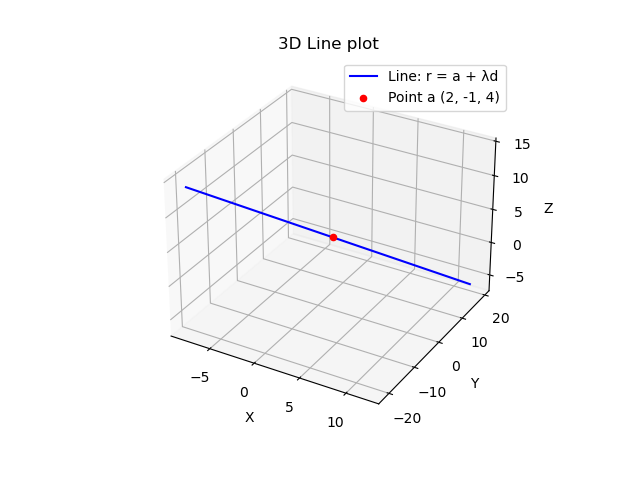
\includegraphics[width = 0.7\columnwidth]{figs/fig1.png}
		\caption{Plot of the 3D line}
		\label{fig1}
	\end{figure}
	\end{center}
\end{frame}
\begin{frame}[fragile]
     \frametitle{Python code for the plot}
\begin{lstlisting}
    import numpy as np
import matplotlib.pyplot as plt

# Given vectors
a = np.array([2, -1, 4])      # point vector
d = np.array([1, 2, -1])      # direction vector

# Parameter lambda values
lambdas = np.linspace(-10, 10, 400)

# Calculate points on the line for each lambda
points = np.array([a + l * d for l in lambdas])
\end{lstlisting}
\end{frame}
\begin{frame}[fragile]
   \frametitle{Python code for the plot}
    \begin{lstlisting}
# Plotting the line in 3D
fig = plt.figure()
ax = fig.add_subplot(111, projection='3d')

ax.plot(points[:, 0], points[:, 1], points[:, 2], label='Line: r = a + λd', color='blue')

# Plot the given point 'a'
ax.scatter(a[0], a[1], a[2], color='red', label='Point a (2, -1, 4)')

ax.set_xlabel('X')
ax.set_ylabel('Y')
ax.set_zlabel('Z')
ax.legend()
plt.title('3D Line plot')
plt.show()
 \end{lstlisting}
\end{frame}
 \begin{figure}
     \centering
     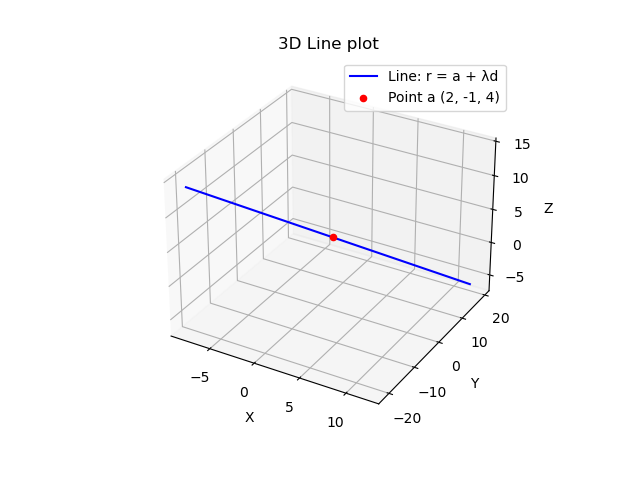
\includegraphics[width=0.7\linewidth]{figs/fig1.png}
     \caption{Plot for the 3D line}
     \label{fig2}
 \end{figure}
\end{document}